%  LaTeX support: latex@mdpi.com 
%  For support, please attach all files needed for compiling as well as the log file, and specify your operating system, LaTeX version, and LaTeX editor.

%=================================================================
\documentclass[journal,article,submit,pdftex,moreauthors]{Definitions/mdpi} 
%\documentclass[preprints,article,submit,pdftex,moreauthors]{Definitions/mdpi} 
% For posting an early version of this manuscript as a preprint, you may use "preprints" as the journal. Changing "submit" to "accept" before posting will remove line numbers.

%--------------------
% Class Options:
%--------------------
%----------
% journal
%----------
% Choose between the following MDPI journals:
% accountaudit, acoustics, actuators, addictions, adhesives, admsci, adolescents, aerobiology, aerospace, agriculture, agriengineering, agrochemicals, agronomy, ai, air, algorithms, allergies, alloys, amh, analytica, analytics, anatomia, anesthres, animals, antibiotics, antibodies, antioxidants, applbiosci, appliedchem, appliedmath, appliedphys, applmech, applmicrobiol, applnano, applsci, aquacj, architecture, arm, arthropoda, arts, asc, asi, astronomy, atmosphere, atoms, audiolres, automation, axioms, bacteria, batteries, bdcc, behavsci, beverages, biochem, bioengineering, biologics, biology, biomass, biomechanics, biomed, biomedicines, biomedinformatics, biomimetics, biomolecules, biophysica, biosensors, biosphere, biotech, birds, blockchains, bloods, blsf, brainsci, breath, buildings, businesses, cancers, carbon, cardiogenetics, catalysts, cells, ceramics, challenges, chemengineering, chemistry, chemosensors, chemproc, children, chips, cimb, civileng, cleantechnol, climate, clinbioenerg, clinpract, clockssleep, cmd, cmtr, coasts, coatings, colloids, colorants, commodities, complications, compounds, computation, computers, condensedmatter, conservation, constrmater, cosmetics, covid, crops, cryo, cryptography, crystals, csmf, ctn, curroncol, cyber, dairy, data, ddc, dentistry, dermato, dermatopathology, designs, devices, diabetology, diagnostics, dietetics, digital, disabilities, diseases, diversity, dna, drones, dynamics, earth, ebj, ecm, ecologies, econometrics, economies, education, eesp, ejihpe, electricity, electrochem, electronicmat, electronics, encyclopedia, endocrines, energies, eng, engproc, ent, entomology, entropy, environments, epidemiologia, epigenomes, esa, est, famsci, fermentation, fibers, fintech, fire, fishes, fluids, foods, forecasting, forensicsci, forests, fossstud, foundations, fractalfract, fuels, future, futureinternet, futureparasites, futurepharmacol, futurephys, futuretransp, galaxies, games, gases, gastroent, gastrointestdisord, gastronomy, gels, genealogy, genes, geographies, geohazards, geomatics, geometry, geosciences, geotechnics, geriatrics, glacies, grasses, greenhealth, gucdd, hardware, hazardousmatters, healthcare, hearts, hemato, hematolrep, heritage, higheredu, highthroughput, histories, horticulturae, hospitals, humanities, humans, hydrobiology, hydrogen, hydrology, hygiene, idr, iic, ijerph, ijfs, ijgi, ijmd, ijms, ijns, ijpb, ijt, ijtm, ijtpp, ime, immuno, informatics, information, infrastructures, inorganics, insects, instruments, inventions, iot, j, jal, jcdd, jcm, jcp, jcs, jcto, jdad, jdb, jeta, jfb, jfmk, jimaging, jintelligence, jlpea, jmahp, jmmp, jmms, jmp, jmse, jne, jnt, jof, joitmc, joma, jop, jor, journalmedia, jox, jpbi, jpm, jrfm, jsan, jtaer, jvd, jzbg, kidney, kidneydial, kinasesphosphatases, knowledge, labmed, laboratories, land, languages, laws, life, lights, limnolrev, lipidology, liquids, literature, livers, logics, logistics, lubricants, lymphatics, machines, macromol, magnetism, magnetochemistry, make, marinedrugs, materials, materproc, mathematics, mca, measurements, medicina, medicines, medsci, membranes, merits, metabolites, metals, meteorology, methane, metrics, metrology, micro, microarrays, microbiolres, microelectronics, micromachines, microorganisms, microplastics, microwave, minerals, mining, mmphys, modelling, molbank, molecules, mps, msf, mti, multimedia, muscles, nanoenergyadv, nanomanufacturing, nanomaterials, ncrna, ndt, network, neuroglia, neurolint, neurosci, nitrogen, notspecified, nursrep, nutraceuticals, nutrients, obesities, oceans, ohbm, onco, oncopathology, optics, oral, organics, organoids, osteology, oxygen, parasites, parasitologia, particles, pathogens, pathophysiology, pediatrrep, pets, pharmaceuticals, pharmaceutics, pharmacoepidemiology, pharmacy, philosophies, photochem, photonics, phycology, physchem, physics, physiologia, plants, plasma, platforms, pollutants, polymers, polysaccharides, populations, poultry, powders, preprints, proceedings, processes, prosthesis, proteomes, psf, psych, psychiatryint, psychoactives, psycholint, publications, purification, quantumrep, quaternary, qubs, radiation, reactions, realestate, receptors, recycling, regeneration, religions, remotesensing, reports, reprodmed, resources, rheumato, risks, robotics, rsee, ruminants, safety, sci, scipharm, sclerosis, seeds, sensors, separations, sexes, signals, sinusitis, siuj, skins, smartcities, sna, societies, socsci, software, soilsystems, solar, solids, spectroscj, sports, standards, stats, std, stresses, surfaces, surgeries, suschem, sustainability, symmetry, synbio, systems, tae, targets, taxonomy, technologies, telecom, test, textiles, thalassrep, therapeutics, thermo, timespace, tomography, tourismhosp, toxics, toxins, transplantology, transportation, traumacare, traumas, tropicalmed, universe, urbansci, uro, vaccines, vehicles, venereology, vetsci, vibration, virtualworlds, viruses, vision, waste, water, wem, wevj, wild, wind, women, world, youth, zoonoticdis

%---------
% article
%---------
% The default type of manuscript is "article", but can be replaced by: 
% abstract, addendum, article, benchmark, book, bookreview, briefcommunication, briefreport, casereport, changes, clinicopathologicalchallenge, comment, commentary, communication, conceptpaper, conferenceproceedings, correction, conferencereport, creative, datadescriptor, discussion, entry, expressionofconcern, extendedabstract, editorial, essay, erratum, fieldguide, hypothesis, interestingimages, letter, meetingreport, monograph, newbookreceived, obituary, opinion, proceedingpaper, projectreport, reply, retraction, review, perspective, protocol, shortnote, studyprotocol, supfile, systematicreview, technicalnote, viewpoint, guidelines, registeredreport, tutorial,  giantsinurology, urologyaroundtheworld
% supfile = supplementary materials

%----------
% submit
%----------
% The class option "submit" will be changed to "accept" by the Editorial Office when the paper is accepted. This will only make changes to the frontpage (e.g., the logo of the journal will get visible), the headings, and the copyright information. Also, line numbering will be removed. Journal info and pagination for accepted papers will also be assigned by the Editorial Office.

%------------------
% moreauthors
%------------------
% If there is only one author the class option oneauthor should be used. Otherwise use the class option moreauthors.

%---------
% pdftex
%---------
% The option pdftex is for use with pdfLaTeX. Remove "pdftex" for (1) compiling with LaTeX & dvi2pdf (if eps figures are used) or for (2) compiling with XeLaTeX.

%=================================================================
% MDPI internal commands - do not modify
\firstpage{1} 
\makeatletter 
\setcounter{page}{\@firstpage} 
\makeatother
\pubvolume{1}
\issuenum{1}
\articlenumber{0}
\pubyear{2025}
\copyrightyear{2025}
%\externaleditor{Firstname Lastname} % More than 1 editor, please add `` and '' before the last editor name
\datereceived{ } 
\daterevised{ } % Comment out if no revised date
\dateaccepted{ } 
\datepublished{ } 
%\datecorrected{} % For corrected papers: "Corrected: XXX" date in the original paper.
%\dateretracted{} % For retracted papers: "Retracted: XXX" date in the original paper.
\hreflink{https://doi.org/} % If needed use \linebreak
%\doinum{}
%\pdfoutput=1 % Uncommented for upload to arXiv.org
%\CorrStatement{yes}  % For updates
%\longauthorlist{yes} % For many authors that exceed the left citation part
%\IsAssociation{yes} % For association journals

%=================================================================
% Add packages and commands here. The following packages are loaded in our class file: fontenc, inputenc, calc, indentfirst, fancyhdr, graphicx, epstopdf, lastpage, ifthen, float, amsmath, amssymb, lineno, setspace, enumitem, mathpazo, booktabs, titlesec, etoolbox, tabto, xcolor, colortbl, soul, multirow, microtype, tikz, totcount, changepage, attrib, upgreek, array, tabularx, pbox, ragged2e, tocloft, marginnote, marginfix, enotez, amsthm, natbib, hyperref, cleveref, scrextend, url, geometry, newfloat, caption, draftwatermark, seqsplit
% cleveref: load \crefname definitions after \begin{document}

%=================================================================
% Please use the following mathematics environments: Theorem, Lemma, Corollary, Proposition, Characterization, Property, Problem, Example, ExamplesandDefinitions, Hypothesis, Remark, Definition, Notation, Assumption
%% For proofs, please use the proof environment (the amsthm package is loaded by the MDPI class).

%=================================================================
% Full title of the paper (Capitalized)
\Title{Title}

% MDPI internal command: Title for citation in the left column
\TitleCitation{Title}

% Author Orchid ID: enter ID or remove command
\newcommand{\orcidauthorA}{0000-0000-0000-000X} % Add \orcidA{} behind the author's name
%\newcommand{\orcidauthorB}{0000-0000-0000-000X} % Add \orcidB{} behind the author's name

% Authors, for the paper (add full first names)
\Author{Firstname Lastname $^{1}$\orcidA{}, Firstname Lastname $^{2}$ and Firstname Lastname $^{2,}$*}

%\longauthorlist{yes}

% MDPI internal command: Authors, for metadata in PDF
\AuthorNames{Firstname Lastname, Firstname Lastname and Firstname Lastname}

% Author citation:  
\AuthorCitation{Lastname, F.; Lastname, F.; Lastname, F.}

% Affiliations / Addresses (Add [1] after \address if there is only one affiliation.)
\address{%
$^{1}$ \quad Affiliation 1; e-mail@e-mail.com\\
$^{2}$ \quad Affiliation 2; e-mail@e-mail.com}

% Contact information of the corresponding author
\corres{Correspondence: e-mail@e-mail.com; Tel.: (optional; include country code; if there are multiple corresponding authors, add author initials) +xx-xxxx-xxx-xxxx (F.L.)}

% Current address and/or shared authorship
%\firstnote{Current address: Affiliation.}  
% Current address should not be the same as any items in the Affiliation section.

%\secondnote{These authors contributed equally to this work.}
% The commands \thirdnote{} till \eighthnote{} are available for further notes.

%\simplesumm{} % Simple summary

%\conference{} % An extended version of a conference paper

% Abstract (Do not insert blank lines, i.e. \\) 
\abstract{Hybrid satellite aerial terrestrial networks (HSATNs) are a promising solution towards tackling coverage and mobility issues in sixth generation (6G) networks.This paper presents a novel transmission scheme in the context of HSATNs,which allows pairs of terrestrial users to be simultaneously served via the satellite and the aerial base station (ABS).To this aim, non-orthogonal multiple access (NOMA) technique is adopted,at the ABS,by applying a rule-based hybrid NOMA and orthogonal multiple access (OMA) schemes.Comparisons between a standalone NOMA-based satellite transmission and the proposed method, reveal that significant sum-rate gains can be harvested under varying system parameters.}

% Keywords
\keyword{keyword 1; keyword 2; keyword 3 (List three to ten pertinent keywords specific to the article; yet reasonably common within the subject discipline.)} 

% The fields PACS, MSC, and JEL may be left empty or commented out if not applicable
%\PACS{J0101}
%\MSC{}
%\JEL{}

%%%%%%%%%%%%%%%%%%%%%%%%%%%%%%%%%%%%%%%%%%
% Only for the journal Diversity
%\LSID{\url{http://}}

%%%%%%%%%%%%%%%%%%%%%%%%%%%%%%%%%%%%%%%%%%
% Only for the journal Applied Sciences
%\featuredapplication{Authors are encouraged to provide a concise description of the specific application or a potential application of the work. This section is not mandatory.}
%%%%%%%%%%%%%%%%%%%%%%%%%%%%%%%%%%%%%%%%%%

%%%%%%%%%%%%%%%%%%%%%%%%%%%%%%%%%%%%%%%%%%
% Only for the journal Data
%\dataset{DOI number or link to the deposited data set if the data set is published separately. If the data set shall be published as a supplement to this paper, this field will be filled by the journal editors. In this case, please submit the data set as a supplement.}
%\datasetlicense{License under which the data set is made available (CC0, CC-BY, CC-BY-SA, CC-BY-NC, etc.)}

%%%%%%%%%%%%%%%%%%%%%%%%%%%%%%%%%%%%%%%%%%
% Only for the journal BioTech, Fishes, Neuroimaging and Toxins
%\keycontribution{The breakthroughs or highlights of the manuscript. Authors can write one or two sentences to describe the most important part of the paper.}

%%%%%%%%%%%%%%%%%%%%%%%%%%%%%%%%%%%%%%%%%%
% Only for the journal Encyclopedia
%\encyclopediadef{For entry manuscripts only: please provide a brief overview of the entry title instead of an abstract.}

%%%%%%%%%%%%%%%%%%%%%%%%%%%%%%%%%%%%%%%%%%
% Different journals have different requirements. Please check the specific journal guidelines in the "Instructions for Authors" on the journal's official website.
%\addhighlights{yes}
%\renewcommand{\addhighlights}{%
%
%\noindent The goal is to increase the discoverability and readability of the article via search engines and other scholars. Highlights should not be a copy of the abstract, but a simple text allowing the reader to quickly and simplified find out what the article is about and what can be cited from it. Each of these parts should be devoted up to 2~bullet points.\vspace{3pt}\\
%\textbf{What are the main findings?}
% \begin{itemize}[labelsep=2.5mm,topsep=-3pt]
% \item First bullet.
% \item Second bullet.
% \end{itemize}\vspace{3pt}
%\textbf{What is the implication of the main finding?}
% \begin{itemize}[labelsep=2.5mm,topsep=-3pt]
% \item First bullet.
% \item Second bullet.
% \end{itemize}
%}

%%%%%%%%%%%%%%%%%%%%%%%%%%%%%%%%%%%%%%%%%%
\begin{document}

%%%%%%%%%%%%%%%%%%%%%%%%%%%%%%%%%%%%%%%%%%
% The order of the section titles is different for some journals. Please refer to the "Instructions for Authors” on the journal homepage.

\section{Introduction}

The sixth generation (6G) network has already been commenced as a new research initiative, following on from the evolving 5G network.This new type of network envisions sophisticated device-to-device (D2D) and machine-to-machine (M2M) communications,innovative artificial intelligence (AI) techniques, Internet of Everything (IoE) applications connecting people, data, things through processes.Interoperability and convergence between terrestrial and satellite infrastructures will be a prerequisite in the 6G networking. Also, the new space era of non-terrestrial networks (NTNs) comprising of aerial networks, low Earth orbit (LEO) and especially very low Earth orbit (VLEO) satellites has emerged, enabling the path to 6G evolution.

Hybrid satellite-terrestrial networks (HSTNs) have been proposed as an efficient approach towards improving spectral efficiency and increasing the users’ reliability all over the world.The available spectrum resources of these networks can be further exploited by adopting the non-orthogonal multiple access (NOMA) principle.However, in the absence of line-of-sight (LoS) conditions, the performance of satellite communication systems is severely deteriorating.

In the context of HSTNs, the unmanned aerial vehicle (UAV)-based communications are expected to improve the performance in various ways.In general, the UAV-aided NOMA  schemes have gained the interest of the academia and the industry for various applications in the beyond 5G networks.Focusing on the scenario where the UAVs are adopted in satellite terrestrial communication networks, they could be employed in the NOMA scheme as an intermediate node for increasing the possibility of obtaining LoS conditions.

All-in-all, and to the best of our knowledge, no studies can be found related to the intelligent integration of aerial and satellite segments in 6G networks by utilizing a hybrid NOMA and orthogonal multiple access (OMA) transmission schemes. Motivated by this observation, in this paper, we propose a novel satellite aerial terrestrial cooperative network scheme, which will be termed SATCON. More specifically, SATCON is formed with the integration of aerial base station (ABS) in the existing satellite network by efficiently combining two unsupervised machine learning (ML) algorithms, namely k-means and k-medoids. Furthermore, the proposed system promotes efficient cooperation between ABS and satellite through an innovative hybrid NOMA/OMA approach, avoiding the waste of resources and energy.Compared to standalone satellite NOMA transmission with optimal user pairing, namely SAT-NOMA, SATCON increases the sum rate and, at the same time, provides higher spectral efficiency for varying satellite channel conditions and ABS bandwidth.
%%%%%%%%%%%%%%%%%%%%%%%%%%%%%%%%%%%%%%%%%%
\section{Materials and Methods}

As shown in Figure~\ref{fig:system_model}, the considered SAGIN consists of $\mathbf{U}$ UAVs denoted by $\mathcal{U} = {1, 2, \dots, U}$ and $\mathbf{S}$ LEO satellites indicated by $\mathcal{S} = {1, 2, \dots, S}$. In addition, $\mathbf{K}$ IoT devices randomly scattered on the ground are represented as $\mathcal{K} = {1, 2, \dots, K}$.

In the downlink, UEs may receive data either directly from the LEO satellite or through a UAV-assisted relaying link over the air-to-ground (A2G) channel. Satellite-side user pairing is first established based on direct downlink transmission, which serves as the reference for subsequent transmission decisions.Under this pairing, UAV-assisted transmission is activated only when it can provide a strict rate improvement over direct satellite delivery. Specifically, if both paired users achieve higher downlink rates via the UAV, UAV-assisted NOMA transmission is employed. If only one user benefits from UAV relaying, UAV-assisted OMA transmission is selectively applied to that user in order to avoid any performance degradation of the other. Otherwise, when UAV-assisted transmission cannot outperform direct satellite transmission for either user, both users are served directly by the satellite.


% Figure 1
\begin{figure}[!htbp]
\centering
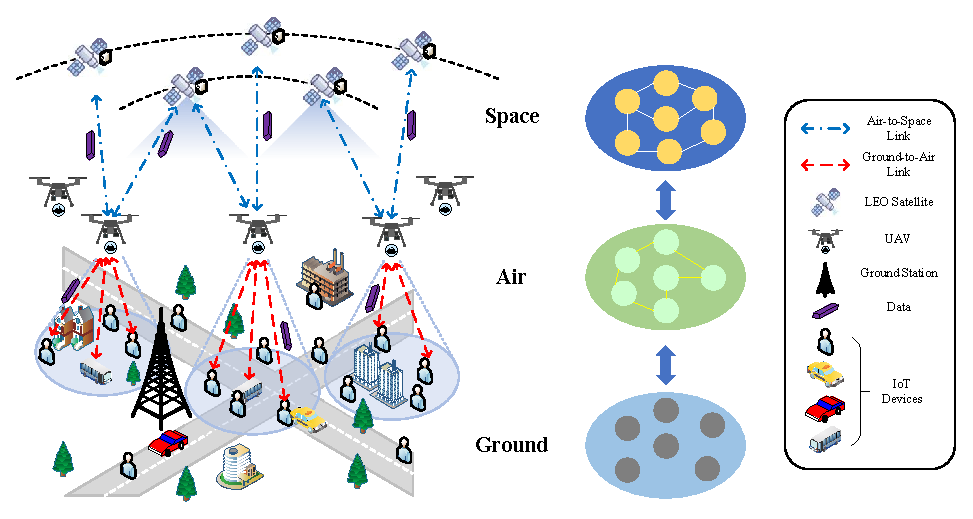
\includegraphics[width=0.95\columnwidth]{Definitions/figure1}
\caption{Illustration of the uplink communication procedure in SAGIN, where UAVs act as aerial aggregators to collect data from spatially distributed IoT devices and subsequently offload the aggregated data to LEO satellites.}
\label{fig:system_model}
\end{figure}

To characterize the downlink transmission options described above, the satellite downlink is modeled using a land mobile satellite(LMS)  channel. The overall channel coefficient between LEO satellite $s$ and UE $i$ is expressed as
\begin{equation}
h_i^s = \sqrt{L_i^s} \cdot g_i^s,
\end{equation}
where $L_i^s$ represents the large-scale free-space path loss given by
\begin{equation}
L_i^s = \left(\frac{c}{4\pi f_c d_i^s}\right)^2,
\end{equation}
with $f_c$ denoting the carrier frequency, $d_i^s$ the satellite-to-UE distance, and $c$ the speed of light.

The small-scale fading coefficient $g_i^s$ follows the Loo model,characterizing the composite fading as a superposition of a dominant line-of-sight (LoS) component and multipath fading
\begin{equation}
g_i^s(t) = A_i(t)e^{j\phi_i(t)} + m_i(t),
\end{equation}
where $A_i(t)$ represents the LoS amplitude with $20\log_{10}A_i(t) \sim \mathcal{N}(\mu, \sigma^2)$, and $m_i(t) = m_{I,i}(t) + jm_{Q,i}(t)$ denotes the multipath component with $m_{I,i}, m_{Q,i} \sim \mathcal{N}(0, \sigma_m^2)$.The parameters are set as $\mu = -1$ dB, $\sigma = 2$ dB, corresponding to a suburban environment.

Furthermore, the Doppler effect induced by satellite motion is captured using the classical Jakes spectrum with maximum Doppler shift $f_D = v f_c / c$, where $v$ denotes the relative velocity between the satellite and UE.

For UAV-assisted transmission, data are forwarded to UEs through an air-to-ground (A2G) link. The channel coefficient between the UAV and UE $i$ is denoted by $h_i^d$ and can be expressed as
\begin{equation}
h_i^d = \sqrt{L_i^{\text{A2G}}} \cdot g_i^d,
\label{eq:channel coefficient}
\end{equation}
where $L_i^{\text{A2G}}$ represents the large-scale path loss and $g_i^d$ denotes the small-scale fading.

Following the elevation-angle-dependent model by Al-Hourani \emph{et al.}~\cite{al2014modeling}, the path loss accounts for probabilistic LoS and NLoS propagation in urban environments. The LoS probability is given by
\begin{equation}
P_{\text{LoS}}(\theta_i) = \frac{1}{1 + a \exp(-b[\theta_i - a])},
\end{equation}
where $\theta_i = \arcsin(H/\sqrt{H^2 + d_i^2})$ is the elevation angle, $H$ is the UAV altitude, $d_i$ is the horizontal distance, and $(a, b)$ are environment-dependent parameters. For urban environments, we adopt $a = 9.61$ and $b = 0.16$~\cite{al2014modeling}.

The composite path loss is then computed as
\begin{equation}
L_i^{\text{A2G}} = P_{\text{LoS}}(\theta_i) \cdot L_i^{\text{LoS}} 
+ [1-P_{\text{LoS}}(\theta_i)] \cdot L_i^{\text{NLoS}},
\end{equation}
where
\begin{align}
L_i^{\text{LoS}}\text{(dB)} &= 20\log_{10}\left(\frac{4\pi f_c d_i^{\text{3D}}}{c}\right) + \eta_{\text{LoS}}, \\
L_i^{\text{NLoS}}\text{(dB)} &= 20\log_{10}\left(\frac{4\pi f_c d_i^{\text{3D}}}{c}\right) + \eta_{\text{NLoS}},
\label{eq:path loss}
\end{align}
with $d_i^{\text{3D}} = \sqrt{H^2 + d_i^2}$ denoting the 3D distance, and $\eta_{\text{LoS}} = 1$ dB, $\eta_{\text{NLoS}} = 20$ dB representing the excessive path loss for LoS and NLoS links, respectively~\cite{al2014modeling}.

It should be emphasized that the downlink rate delivered to a UE via UAV-assisted relaying is jointly determined by the A2G access link and the satellite-to-UAV (S2A) backhaul. Since the UAV can only forward the data it receives from the satellite, the capacity of the S2A backhaul may limit the effective downlink rate, preventing UAV-assisted transmission from consistently outperforming direct satellite delivery.

All downlink links are assumed to be impaired by additive white Gaussian noise (AWGN). These channel characteristics explain why UAV-assisted relaying may provide significant rate gains for some users while offering no advantage for others, thereby motivating rate-based downlink transmission mode selection.

\subsection{ABS placement process}

The ABS placement is performed prior to the hybrid transmission decision, since the A2G channel characteristics—and consequently the achievable UAV-assisted rates—are fundamentally determined by the ABS position. Without an appropriately optimized ABS location, the hybrid NOMA/OMA decision would be restricted to a limited set of feasible transmission options, leading to suboptimal system performance.

To facilitate effective hybrid NOMA/OMA downlink decision-making, the ABS placement is designed as a performance-aware structural optimization step rather than an isolated objective. Specifically, the three-dimensional ABS position $\mathbf{p} = (x_1^{p}, y_1^{p}, z_1^{p})$ is optimized to enhance the quality of the air-to-ground (A2G) channels, which directly determine the achievable UAV-assisted transmission rates. By improving the overall A2G channel conditions through position optimization, the proposed placement strategy enlarges the set of users for which UAV-assisted transmission can provide rate advantages over direct satellite delivery, thereby enabling more effective hybrid NOMA/OMA transmission decisions in the subsequent stage.It is worth noting that the placement optimization does not determine the transmission mode itself, but rather provides a favorable channel structure upon which the subsequent rate-based hybrid decision operates.
Based on the above considerations, the ABS placement is formulated as a preliminary, performance-aware optimization step that aims to enhance the air-to-ground (A2G) channel conditions prior to the hybrid transmission decision. Specifically, the three-dimensional ABS position $\mathbf{p} \in W$ is determined by maximizing the aggregate A2G downlink rate experienced by terrestrial users, which is expressed as
\begin{equation}
\underset{\mathbf{p} \in W}{\arg\max} \sum_{i \in \mathcal{K}} R_i^d(\mathbf{p}),
\label{eq:abs_placement_obj}
\end{equation}
where $W$ denotes the feasible spatial region for ABS deployment, and $R_i^d(\mathbf{p})$ represents the achievable A2G downlink rate for $\mathrm{IoT}_i$ when the ABS is positioned at $\mathbf{p}$. Since the subsequent hybrid NOMA/OMA transmission decision involves discrete user pairing and mode selection, a continuous and differentiable surrogate is adopted during the placement phase. In particular, the OMA transmission rate is used as a proxy for the A2G channel quality, given by
\begin{equation}
R_i^d(\mathbf{p}) = B_d \log_2 \left( 1 + P_d \Gamma_i^d(\mathbf{p}) \right),
\label{eq:oma_surrogate}
\end{equation}
where $B_d$ denotes the allocated A2G bandwidth, $P_d$ is the transmission power of the ABS, and $\Gamma_i^d(\mathbf{p})$ is the channel gain experienced by $\mathrm{IoT}_i$, which explicitly depends on the ABS position $\mathbf{p}$. 
By optimizing \eqref{eq:abs_placement_obj} with respect to $\mathbf{p}$, the proposed placement strategy improves the overall A2G channel quality, thereby providing a favorable rate landscape for the subsequent hybrid NOMA/OMA downlink decision.

The channel gain $\Gamma_i^d(\mathbf{p})$ is determined by the A2G channel model, and depends explicitly on the ABS position $\mathbf{p}$ through the elevation-angle-dependent path loss and the associated line-of-sight probability. In particular, both the horizontal distance between the ABS and $\mathrm{IoT}_i$ and the ABS altitude jointly influence the large-scale attenuation, which in turn affects the achievable A2G downlink rate.


The ABS position is restricted by the physical service area and practical deployment constraints of the considered system. Specifically, the horizontal coordinates of the ABS are confined within the coverage region of radius $R_{\text{cov}}$, while the altitude is limited to a feasible range $[z_{\text{min}}, z_{\text{max}}]$ to ensure reliable communication performance and compliance with regulatory requirements. These constraints can be expressed as
\begin{equation}
\begin{aligned}
    -R_{\text{cov}} &\leq x_1^{p} \leq R_{\text{cov}}, \\
    -R_{\text{cov}} &\leq y_1^{p} \leq R_{\text{cov}}, \\
    z_{\text{min}} &\leq z_1^{p} \leq z_{\text{max}},
\end{aligned}
\label{eq:position_constraints}
\end{equation}
where $R_{\text{cov}}$ denotes the horizontal coverage radius of the service area, and $[z_{\text{min}}, z_{\text{max}}]$ represents the permissible altitude range for ABS deployment, typically set to $[50~\text{m}, 500~\text{m}]$.

The ABS placement problem in~\eqref{eq:abs_placement_obj} is solved using the Limited-memory Broyden--Fletcher--Goldfarb--Shanno with Box constraints (L-BFGS-B) algorithm, which is suitable for bound-constrained nonlinear optimization. 
Starting from an initial position $\mathbf{p}_0$ defined by the geometric centroid of the user distribution in the horizontal plane with a default altitude of $100~\text{m}$, the algorithm iteratively updates the ABS location based on gradient information until convergence. The convergence tolerance is set to $\epsilon = 10^{-6}$ on the objective function value, with a maximum iteration limit of $100$ to ensure computational efficiency.

During the placement phase, the OMA rate in~\eqref{eq:oma_surrogate} is adopted as a continuous and differentiable surrogate, since the hybrid NOMA/OMA transmission scheme involves discrete user pairing and successive interference cancellation (SIC) operations that are not suitable for gradient-based optimization. The use of the OMA rate allows the placement optimization to focus on improving the A2G channel conditions without imposing any transmission mode decisions.

The optimized ABS position obtained from this procedure is subsequently used as the deployment configuration for the hybrid NOMA/OMA downlink transmission.

\subsection{Satellite NOMA transmission}

For the satellite transmission, each $M T_l \ (1 \le l \le N)$ periodically reports the channel state information (CSI) of the LMS channel to the satellite that receives the complex channel coefficient $h_l^s$ and calculates the channel gain including additional gains, losses, and the noise power of the satellite receiver $N_s$ as
\begin{equation}
\Gamma_{l}^{s}
= \frac{G_{t}^{s} G_{r}^{s}}{L_{l}^{\mathrm{FS}} N_{s}} \, |h_{l}^{s}|^{2}.
\end{equation}

The satellite aims to create $K$ pairs of MTs, where each pair will share the same sub-channel in the power and time domain, assigning different power allocation factors of the total satellite power $P_s$ to each MT belonging to a pair. Towards this end, a NOMA optimal user pairing policy is adopted, where the satellite sorts the MTs in ascending order by the channel gain $\Gamma_1^{s} \le \Gamma_2^{s} \le \cdots \le \Gamma_{2K}^{s}$ and matches the user $MT_k$ with the user $MT_{2K-k+1}$, for $1 \le k \le K$.Hence, each pair consists of the strong satellite channel user $MT_j^s$, and the weak satellite  channel user $MT_i^s$, with channel gains $\Gamma_j^{s} \ge \Gamma^{s}$,respectively.

The optimal power allocation factor $\beta_j^s$ can be calculated by the following expression
\begin{equation}
\beta_{j}^{s}
= \frac{\sqrt{1 + \Gamma_{i}^{s} P_{s}} - 1}{\Gamma_{i}^{s} P_{s}}.
\label{power allocation}
\end{equation}

According to the principle of NOMA, $MT_i^s$ will immediately decode its own signal by the received satellite signal, while $MT_j^s$ should first estimate the signal of the $MT_i^s$ and then perform successive interference cancellation (SIC) to retrieve its own signal.The achievable rates of $MT_j^s$ and $MT_i^s$ are
\begin{equation}
R_{j}^{s}
= \frac{B_{s}}{K} \log_{2}\!\left( 1 + \beta_{j}^{s} P_{s} \Gamma_{j}^{s} \right),
\label{achievable rates j}
\end{equation}
\begin{equation}
R_{i}^{s}
= \frac{B_{s}}{K} \log_{2}\!\left(
1 + \frac{(1 - \beta_{j}^{s}) P_{s} \Gamma_{i}^{s}}{\beta_{j}^{s} P_{s} \Gamma_{i}^{s} + 1}
\right).
\label{achievable rates i}
\end{equation}

\subsection{ABS hybrid NOMA/OMA transmission}

As described previously, ABS is integrated into the satellite network to improve the QoS of terrestrial users. Towards this end, the ABS should first receive and decode the NOMA superimposed signals of each pair of MTs via the S2A channel. The S2A channel gain can be expressed as
\begin{equation}
\Lambda_{sd}
= \frac{G_{t}^{s} G_{r}^{sd}}{L_{sd}^{\mathrm{FS}} N_{sd}}.
\end{equation}
The maximum achievable decoding rates which succeed by the ABS through the S2A channel for each $MT_j^s$ and $MT_i^s$ in pair are
\begin{equation}
R_{j}^{sd}
= \frac{B_{s}}{K} \log_{2}\!\left( 1 + \beta_{j}^{s} P_{s} \Lambda_{sd} \right),
\end{equation}
\begin{equation}
R_{i}^{sd}
= \frac{B_{s}}{K} \log_{2}\!\left(
1 + \frac{(1 - \beta_{j}^{s}) P_{s} \Lambda_{sd}}
{\beta_{j}^{s} P_{s} \Lambda_{sd} + 1}
\right).
\end{equation}

Note that, the ABS obtains all the pair indices from the VLEO through a dedicated control channel to identify the users comprising each pair and their role, e.g., strong or weak satellite channel users. Also, the ABS acquires the achievable rate $R_l^s$ of each $MT_l$ with the satellite, through the same channel.

Next, the ABS should forward the decoded signals to the MTs through the A2G channel, utilizing the proposed hybrid NOMA/OMA transmission scheme. Consequently, we consider that each $MT_l$ reports the CSI of the corresponding A2G link to the ABS. Therefore, the ABS calculates the channel gain of the A2G link for each M Tl as follows
\begin{equation}
\Gamma_{l}^{d}
= \frac{G_{t}^{d} G_{r}^{d}}{L_{l}^{\mathrm{A2G}}(h, r_{l}) \, N_{d}} \, |h_{l}^{d}|^{2}.
\end{equation}

Following the same NOMA user pairing policy as the VLEO, the ABS forms $K$ MT pairs, considering now the channel gains of the A2G links. Therefore, each pair consists of the strong A2G channel user $MT_j^d$, and the weak A2G channel user $MT_i^d$, where $\Gamma_{j}^{d} \ge \Gamma_{i}^{d}$. Subsequently, calculates the optimal power allocation factor $\beta_j^d$ for the $MT_j^d$ by replacing $s$ with $d$ in expression \ref{power allocation}.Also, the achievable rates in NOMA, $R_j^d$ and $MT_i^d$,are given by the expressions \ref{achievable rates j} and \ref{achievable rates i}, respectively, by replacing again $s$ with $d$.The rates that ABS can offer to $MT_j^d$ and $MT_i^d$, utilizing the NOMA technique, are $R_{j}^{dn} = \min\left( R_{j}^{d},\, R_{j}^{sd} \right)$ and $R_{i}^{dn} = \min\left( R_{i}^{d},\, R_{i}^{sd} \right)$,respectively.

Lastly, the ABS has to decide whether it is profitable for each pair of MTs to transmit the superimposed signal or to transmit only the signal of one MT of each pair utilizing the OMA technique. Also, the ABS can avoid forwarding the satellite signals if the ABS transmission is not profitable for both MTs in pair. Therefore, the achievable rate that each $MT_l$ can achieve from the ABS through OMA, is equal to
\begin{equation}
R_{l}^{o}
= \frac{B_{d}}{K} \log_{2}\!\left( 1 + P_{d} \Gamma_{l}^{d} \right).
\end{equation}
Each $MT_l$ will experience higher rates if the ABS uses OMA, i.e., $R_{l}^{o} \ge R_{l}^{d}$, since the same bandwidth as NOMA is allocated for OMA transmission, and whole $P_d$ is allocated to $MT_l$. However, the maximum achievable OMA rate of $MT_l$ is restricted by the expression $R_{l}^{do} = \min\left( R_{l}^{o},\, R_{l}^{sd} \right)$,since the ABS may provide a higher rate to the $MT_l$,but the rate at which ABS decoded its signal from the VLEO is lower and vice versa. There are four different cases that the ABS considers for each MT pair
\begin{itemize}
\item	$\bf{if}$ $R_{i}^{s} < R^{dn}_i$ $\bf{and}$ $R_{j}^{s} < R_{j}^{dn}$: In this case, the pair of MTs formed by the ABS profits from the NOMA transmission as both MTs achieve greater rates if served from the ABS instead of the satellite.
\item	$\bf{if}$ $R_{i}^{s} < R^{dn}_i$ $\bf{and}$ $R_{j}^{s} \ge R_{j}^{dn}$: In this case, only $MT_i^d$ profits from the ABS transmission. Thus, the ABS  utilizes OMA and transmits only to $MT_i^d$ or the timeslot allocated to this pair. $MT_i^d$ achieves a rate equal to $R_i^{do}$.
\item	$\bf{if}$ $R_{i}^{s} \ge R^{dn}_i$ $\bf{and}$ $R_{j}^{s} < R_{j}^{dn}$: In this case, only $MT_j^d$ profits from the ABS transmission. Therefore, the ABS utilizes OMA and transmits only to $MT_j^d$ for the timeslot allocated to this pair. $MT_j^d$ achieves a rate equal to $R_i^{do}$.
\item  Otherwise, the communication for this MT pair is not profitable and ABS does not transmit to these pair of users in order to save resources.
\end{itemize}
%%%%%%%%%%%%%%%%%%%%%%%%%%%%%%%%%%%%%%%%%%
\section{Results}

This section may be divided by subheadings. It should provide a concise and precise description of the experimental results, their interpretation as well as the experimental conclusions that can be drawn.
\subsection{Subsection}
\subsubsection{Subsubsection}

Bulleted lists look like this:
\begin{itemize}
\item	First bullet;
\item	Second bullet;
\item	Third bullet.
\end{itemize}

Numbered lists can be added as follows:
\begin{enumerate}
\item	First item; 
\item	Second item;
\item	Third item.
\end{enumerate}

The text continues here.

\subsection{Figures, Tables and Schemes}

All figures and tables should be cited in the main text as Figure~\ref{fig1}, Table~\ref{tab1}, etc.

\begin{figure}[H]
%\isPreprints{\centering}{} % Only used for preprints
\includegraphics[width=4.0 cm]{Definitions/logo-mdpi}
\caption{This is a figure. Schemes follow the same formatting.\label{fig1}}
\end{figure}   
\unskip

\begin{table}[H] 
%\small % Change table font size
\caption{This is a table caption. Tables should be placed in the main text near to the first time they are~cited.\label{tab1}}
%\isPreprints{\centering}{} % Only used for preprints
\begin{tabularx}{\textwidth}{CCC}
\toprule
\textbf{Title 1}	& \textbf{Title 2}	& \textbf{Title 3}\\
\midrule
Entry 1		& Data			& Data\\
Entry 2		& Data			& Data \textsuperscript{1}\\
\bottomrule
\end{tabularx}

\noindent{\footnotesize{\textsuperscript{1} Tables may have a footer.}}
\end{table}

The text continues here (Figure~\ref{fig2} and Table~\ref{tab2}).

% Example of a figure that spans the whole page width and with subfigures. The same concept works for tables, too.
\begin{figure}[H]
%\isPreprints{} % If the paper is ``preprints'', please uncomment this parenthesis.
\subfloat[\centering]{\includegraphics[width=7.0cm]{Definitions/logo-mdpi}}
%\hfill
\subfloat[\centering]{\includegraphics[width=7.0cm]{Definitions/logo-mdpi}}\\
\subfloat[\centering]{\includegraphics[width=7.0cm]{Definitions/logo-mdpi}}
%\hfill
\subfloat[\centering]{\includegraphics[width=7.0cm]{Definitions/logo-mdpi}}
%\isPreprints{} % If the paper is ``preprints'', please uncomment this parenthesis.
\caption{This is a wide figure. Schemes follow the same formatting. If there are multiple panels, they should be listed as: (\textbf{a}) Description of what is contained in the first panel. (\textbf{b}) Description of what is contained in the second panel. (\textbf{c}) Description of what is contained in the third panel. (\textbf{d}) Description of what is contained in the fourth panel. Figures should be placed in the main text near to the first time they are cited. A caption on a single line should be centered.\label{fig2}}
\end{figure} 

\begin{table}[H]
\caption{This is a wide table.\label{tab2}}
%\isPreprints{\centering} % If the paper is ``preprints'', please uncomment this parenthesis.
%\isPreprints{\begin{tabularx}{\textwidth}{CCCC}} % If the paper is ``preprints'', please uncomment this parenthesis.
			\toprule
			\textbf{Title 1}	& \textbf{Title 2}	& \textbf{Title 3}     & \textbf{Title 4}\\
			\midrule
\multirow[m]{3}{*}{Entry 1 *}	& Data			& Data			& Data\\
			  	                   & Data			& Data			& Data\\
			             	      & Data			& Data			& Data\\
                   \midrule
\multirow[m]{3}{*}{Entry 2}    & Data			& Data			& Data\\
			  	                  & Data			& Data			& Data\\
			             	     & Data			& Data			& Data\\
			\bottomrule
		\end{tabularx}
%		\isPreprints{} % If the paper is ``preprints'', please uncomment this parenthesis.
	\noindent{\footnotesize{* Tables may have a footer.}}
\end{table}

%\begin{listing}[H]
%\caption{Title of the listing}
%\rule{\columnwidth}{1pt}
%\raggedright Text of the listing. In font size footnotesize, small, or normalsize. Preferred format: left aligned and single spaced. Preferred border format: top border line and bottom border line.
%\rule{\columnwidth}{1pt}
%\end{listing}

Text.

Text.

\subsection{Formatting of Mathematical Components}

This is the example 1 of equation:
\begin{linenomath}
\begin{equation}
a = 1,
\end{equation}
\end{linenomath}
the text following an equation need not be a new paragraph. Please punctuate equations as regular text.
%% If the documentclass option "submit" is chosen, please insert a blank line before and after any math environment (equation and eqnarray environments). This ensures correct linenumbering. The blank line should be removed when the documentclass option is changed to "accept" because the text following an equation should not be a new paragraph.

This is the example 2 of equation:
%\isPreprints{} % If the paper is ``preprints'', please uncomment this parenthesis.
\begin{equation}
a = b + c + d + e + f + g + h + i + j + k + l + m + n + o + p + q + r + s + t + u + v + w + x + y + z
\end{equation}
%\isPreprints{} % If the paper is ``preprints'', please uncomment this parenthesis.

%% Example of a page in landscape format (with table and table footnote).
%\startlandscape
%\begin{table}[H] %% Table in wide page
%%\isPreprints{\centering}{} % This command is only used for ``preprints''.
%\caption{This is a very wide table.\label{tab3}}
%	\begin{tabularx}{\textwidth}{CCCC}
%		\toprule
%		\textbf{Title 1}	& \textbf{Title 2}	& \textbf{Title 3}	& \textbf{Title 4}\\
%		\midrule
%		Entry 1		& Data			& Data			& This cell has some longer content that runs over two lines.\\
%		Entry 2		& Data			& Data			& Data\textsuperscript{1}\\
%		\bottomrule
%	\end{tabularx}
%%\isPreprints{}{% This command is only used for ``preprints''.
%	\begin{adjustwidth}{+\extralength}{0cm}
%%} % If the paper is ``preprints'', please uncomment this parenthesis.
%		\noindent\footnotesize{\textsuperscript{1} This is a table footnote.}
%%\isPreprints{}{% This command is only used for ``preprints''.
%	\end{adjustwidth}
%%} % If the paper is ``preprints'', please uncomment this parenthesis.
%\end{table}
%\finishlandscape

Please punctuate equations as regular text. Theorem-type environments (including propositions, lemmas, corollaries etc.) can be formatted as follows:
%% Example of a theorem:
\begin{Theorem}
Example text of a theorem.
\end{Theorem}

The text continues here. Proofs must be formatted as follows:

%% Example of a proof:
\begin{proof}[Proof of Theorem 1]
Text of the proof. Note that the phrase ``of Theorem 1'' is optional if it is clear which theorem is being referred to.
\end{proof}
The text continues here.

%%%%%%%%%%%%%%%%%%%%%%%%%%%%%%%%%%%%%%%%%%
\section{Discussion}

Authors should discuss the results and how they can be interpreted from the perspective of previous studies and of the working hypotheses. The findings and their implications should be discussed in the broadest context possible. Future research directions may also be highlighted.

%%%%%%%%%%%%%%%%%%%%%%%%%%%%%%%%%%%%%%%%%%
\section{Conclusions}

This section is not mandatory, but can be added to the manuscript if the discussion is unusually long or complex.

%%%%%%%%%%%%%%%%%%%%%%%%%%%%%%%%%%%%%%%%%%
\section{Patents}

This section is not mandatory, but may be added if there are patents resulting from the work reported in this manuscript.

%%%%%%%%%%%%%%%%%%%%%%%%%%%%%%%%%%%%%%%%%%
\vspace{6pt} 

%%%%%%%%%%%%%%%%%%%%%%%%%%%%%%%%%%%%%%%%%%
%% optional
%\supplementary{The following supporting information can be downloaded at:  \linksupplementary{s1}, Figure S1: title; Table S1: title; Video S1: title.}

% Only for journal Methods and Protocols:
% If you wish to submit a video article, please do so with any other supplementary material.
% \supplementary{The following supporting information can be downloaded at: \linksupplementary{s1}, Figure S1: title; Table S1: title; Video S1: title. A supporting video article is available at doi: link.}

% Only used for preprtints:
% \supplementary{The following supporting information can be downloaded at the website of this paper posted on \href{https://www.preprints.org/}{Preprints.org}.}

% Only for journal Hardware:
% If you wish to submit a video article, please do so with any other supplementary material.
% \supplementary{The following supporting information can be downloaded at: \linksupplementary{s1}, Figure S1: title; Table S1: title; Video S1: title.\vspace{6pt}\\
%\begin{tabularx}{\textwidth}{lll}
%\toprule
%\textbf{Name} & \textbf{Type} & \textbf{Description} \\
%\midrule
%S1 & Python script (.py) & Script of python source code used in XX \\
%S2 & Text (.txt) & Script of modelling code used to make Figure X \\
%S3 & Text (.txt) & Raw data from experiment X \\
%S4 & Video (.mp4) & Video demonstrating the hardware in use \\
%... & ... & ... \\
%\bottomrule
%\end{tabularx}
%}

%%%%%%%%%%%%%%%%%%%%%%%%%%%%%%%%%%%%%%%%%%
\authorcontributions{For research articles with several authors, a short paragraph specifying their individual contributions must be provided. The following statements should be used ``Conceptualization, X.X. and Y.Y.; methodology, X.X.; software, X.X.; validation, X.X., Y.Y. and Z.Z.; formal analysis, X.X.; investigation, X.X.; resources, X.X.; data curation, X.X.; writing---original draft preparation, X.X.; writing---review and editing, X.X.; visualization, X.X.; supervision, X.X.; project administration, X.X.; funding acquisition, Y.Y. All authors have read and agreed to the published version of the manuscript.'', please turn to the  \href{http://img.mdpi.org/data/contributor-role-instruction.pdf}{CRediT taxonomy} for the term explanation. Authorship must be limited to those who have contributed substantially to the work~reported.}

\funding{Please add: ``This research received no external funding'' or ``This research was funded by NAME OF FUNDER grant number XXX.'' and  and ``The APC was funded by XXX''. Check carefully that the details given are accurate and use the standard spelling of funding agency names at \url{https://search.crossref.org/funding}, any errors may affect your future funding.}

\institutionalreview{In this section, you should add the Institutional Review Board Statement and approval number, if relevant to your study. You might choose to exclude this statement if the study did not require ethical approval. Please note that the Editorial Office might ask you for further information. Please add “The study was conducted in accordance with the Declaration of Helsinki, and approved by the Institutional Review Board (or Ethics Committee) of NAME OF INSTITUTE (protocol code XXX and date of approval).” for studies involving humans. OR “The animal study protocol was approved by the Institutional Review Board (or Ethics Committee) of NAME OF INSTITUTE (protocol code XXX and date of approval).” for studies involving animals. OR “Ethical review and approval were waived for this study due to REASON (please provide a detailed justification).” OR “Not applicable” for studies not involving humans or animals.}

\informedconsent{Any research article describing a study involving humans should contain this statement. Please add ``Informed consent was obtained from all subjects involved in the study.'' OR ``Patient consent was waived due to REASON (please provide a detailed justification).'' OR ``Not applicable'' for studies not involving humans. You might also choose to exclude this statement if the study did not involve humans.

Written informed consent for publication must be obtained from participating patients who can be identified (including by the patients themselves). Please state ``Written informed consent has been obtained from the patient(s) to publish this paper'' if applicable.}

\dataavailability{We encourage all authors of articles published in MDPI journals to share their research data. In this section, please provide details regarding where data supporting reported results can be found, including links to publicly archived datasets analyzed or generated during the study. Where no new data were created, or where data is unavailable due to privacy or ethical restrictions, a statement is still required. Suggested Data Availability Statements are available in section ``MDPI Research Data Policies'' at \url{https://www.mdpi.com/ethics}.} 

% Only for journal Drones
%\durcstatement{Current research is limited to the [please insert a specific academic field, e.g., XXX], which is beneficial [share benefits and/or primary use] and does not pose a threat to public health or national security. Authors acknowledge the dual-use potential of the research involving xxx and confirm that all necessary precautions have been taken to prevent potential misuse. As an ethical responsibility, authors strictly adhere to relevant national and international laws about DURC. Authors advocate for responsible deployment, ethical considerations, regulatory compliance, and transparent reporting to mitigate misuse risks and foster beneficial outcomes.}

% Only for journal Nursing Reports
%\publicinvolvement{Please describe how the public (patients, consumers, carers) were involved in the research. Consider reporting against the GRIPP2 (Guidance for Reporting Involvement of Patients and the Public) checklist. If the public were not involved in any aspect of the research add: ``No public involvement in any aspect of this research''.}
%
%% Only for journal Nursing Reports
%\guidelinesstandards{Please add a statement indicating which reporting guideline was used when drafting the report. For example, ``This manuscript was drafted against the XXX (the full name of reporting guidelines and citation) for XXX (type of research) research''. A complete list of reporting guidelines can be accessed via the equator network: \url{https://www.equator-network.org/}.}
%
%% Only for journal Nursing Reports
%\useofartificialintelligence{Please describe in detail any and all uses of artificial intelligence (AI) or AI-assisted tools used in the preparation of the manuscript. This may include, but is not limited to, language translation, language editing and grammar, or generating text. Alternatively, please state that “AI or AI-assisted tools were not used in drafting any aspect of this manuscript”.}

\acknowledgments{In this section you can acknowledge any support given which is not covered by the author contribution or funding sections. This may include administrative and technical support, or donations in kind (e.g., materials used for experiments). Where GenAI has been used for purposes such as generating text, data, or graphics, or for study design, data collection, analysis, or interpretation of data, please add “During the preparation of this manuscript/study, the author(s) used [tool name, version information] for the purposes of [description of use]. The authors have reviewed and edited the output and take full responsibility for the content of this publication.”}

\conflictsofinterest{Declare conflicts of interest or state ``The authors declare no conflicts of interest.'' Authors must identify and declare any personal circumstances or interest that may be perceived as inappropriately influencing the representation or interpretation of reported research results. Any role of the funders in the design of the study; in the collection, analyses or interpretation of data; in the writing of the manuscript; or in the decision to publish the results must be declared in this section. If there is no role, please state ``The funders had no role in the design of the study; in the collection, analyses, or interpretation of data; in the writing of the manuscript; or in the decision to publish the results''.} 

%%%%%%%%%%%%%%%%%%%%%%%%%%%%%%%%%%%%%%%%%%
%% Optional

%% Only for journal Encyclopedia
%\entrylink{The Link to this entry published on the encyclopedia platform.}

\abbreviations{Abbreviations}{
The following abbreviations are used in this manuscript:
\\

\noindent 
\begin{tabular}{@{}ll}
MDPI & Multidisciplinary Digital Publishing Institute\\
DOAJ & Directory of open access journals\\
TLA & Three letter acronym\\
LD & Linear dichroism
\end{tabular}
}

%%%%%%%%%%%%%%%%%%%%%%%%%%%%%%%%%%%%%%%%%%
%% Optional
\appendixtitles{no} % Leave argument "no" if all appendix headings stay EMPTY (then no dot is printed after "Appendix A"). If the appendix sections contain a heading then change the argument to "yes".
\appendixstart
\appendix
\section[\appendixname~\thesection]{}
\subsection[\appendixname~\thesubsection]{}
The appendix is an optional section that can contain details and data supplemental to the main text---for example, explanations of experimental details that would disrupt the flow of the main text but nonetheless remain crucial to understanding and reproducing the research shown; figures of replicates for experiments of which representative data are shown in the main text can be added here if brief, or as Supplementary Data. Mathematical proofs of results not central to the paper can be added as an appendix.

\begin{table}[H] 
\caption{This is a table caption.\label{tab5}}
%\newcolumntype{C}{>{\centering\arraybackslash}X}
\begin{tabularx}{\textwidth}{CCC}
\toprule
\textbf{Title 1}	& \textbf{Title 2}	& \textbf{Title 3}\\
\midrule
Entry 1		& Data			& Data\\
Entry 2		& Data			& Data\\
\bottomrule
\end{tabularx}
\end{table}

\section[\appendixname~\thesection]{}
All appendix sections must be cited in the main text. In the appendices, Figures, Tables, etc. should be labeled, starting with ``A''---e.g., Figure A1, Figure A2, etc.

%%%%%%%%%%%%%%%%%%%%%%%%%%%%%%%%%%%%%%%%%%
%\isPreprints{} % If the paper is ``preprints'', please uncomment this parenthesis.
%\printendnotes[custom] % Un-comment to print a list of endnotes

\reftitle{References}

% Please provide the correct journal abbreviation (e.g. according to the “List of Title Word Abbreviations” http://www.issn.org/services/online-services/access-to-the-ltwa/).
% Citations and References in Supplementary files are permitted provided that they also appear in the reference list here. 

%=====================================
% References, variant A: external bibliography
%=====================================
% \bibliography{your_external_BibTeX_file}

%=====================================
% References, variant B: internal bibliography
%=====================================

% ACS format
\begin{thebibliography}{999}
% Reference 1
\bibitem{ref-journal}
Author~1, T. The title of the cited article. {\em Journal Abbreviation} {\bf 2008}, {\em 10}, 142--149.
% Reference 2
\bibitem{ref-book1}
Author~2, L. The title of the cited contribution. In {\em The Book Title}; Editor 1, F., Editor 2, A., Eds.; Publishing House: City, Country, 2007; pp. 32--58.
% Reference 3
\bibitem{ref-book2}
Author 1, A.; Author 2, B. \textit{Book Title}, 3rd ed.; Publisher: Publisher Location, Country, 2008; pp. 154--196.
% Reference 4
\bibitem{ref-unpublish}
Author 1, A.B.; Author 2, C. Title of Unpublished Work. \textit{Abbreviated Journal Name} year, \textit{phrase indicating stage of publication (submitted; accepted; in press)}.
% Reference 5
\bibitem{ref-url}
Title of Site. Available online: URL (accessed on Day Month Year).
% Reference 6
\bibitem{ref-proceeding}
Author 1, A.B.; Author 2, C.D.; Author 3, E.F. Title of presentation. In Proceedings of the Name of the Conference, Location of Conference, Country, Date of Conference (Day Month Year); Abstract Number (optional), Pagination (optional).
% Reference 7
\bibitem{ref-thesis}
Author 1, A.B. Title of Thesis. Level of Thesis, Degree-Granting University, Location of University, Date of Completion.
% Reference 8
\bibitem{al2014modeling}
Al-Hourani, A.; Kandeepan, S.; Lardner, S.Optimal LAP Altitude for Maximum Coverage.{\em IEEE Wireless Commun. Lett.} {\bf 2014}, {\em 3}, 569--572.

\end{thebibliography}

% If authors have biography, please use the format below
%\section*{Short Biography of Authors}
%\bio
%{\raisebox{-0.35cm}{\includegraphics[width=3.5cm,height=5.3cm,clip,keepaspectratio]{Definitions/author1.pdf}}}
%{\textbf{Firstname Lastname} Biography of first author}
%
%\bio
%{\raisebox{-0.35cm}{\includegraphics[width=3.5cm,height=5.3cm,clip,keepaspectratio]{Definitions/author2.jpg}}}
%{\textbf{Firstname Lastname} Biography of second author}

% For the MDPI journals use author-date citation, please follow the formatting guidelines on http://www.mdpi.com/authors/references
% To cite two works by the same author: \citeauthor{ref-journal-1a} (\citeyear{ref-journal-1a}, \citeyear{ref-journal-1b}). This produces: Whittaker (1967, 1975)
% To cite two works by the same author with specific pages: \citeauthor{ref-journal-3a} (\citeyear{ref-journal-3a}, p. 328; \citeyear{ref-journal-3b}, p.475). This produces: Wong (1999, p. 328; 2000, p. 475)

%%%%%%%%%%%%%%%%%%%%%%%%%%%%%%%%%%%%%%%%%%
%% for journal Sci
%\reviewreports{\\
%Reviewer 1 comments and authors’ response\\
%Reviewer 2 comments and authors’ response\\
%Reviewer 3 comments and authors’ response
%}
%%%%%%%%%%%%%%%%%%%%%%%%%%%%%%%%%%%%%%%%%%
\PublishersNote{}
%\isPreprints{} % If the paper is ``preprints'', please uncomment this parenthesis.
\end{document}

